\documentclass[a4paper,12pt]{article}
\usepackage[utf8]{inputenc}
\usepackage[french]{babel}
\usepackage[T1]{fontenc}
\usepackage[top=2cm,bottom=2cm,left=2cm,right=2cm]{geometry}
\usepackage{graphicx}

\usepackage{hyperref}
\usepackage{listings}
\usepackage{array}
\usepackage[ruled,vlined]{algorithm2e}
\usepackage{algpseudocode}
\usepackage{amsmath}
\usepackage{tikz} 
\usepackage{caption}
\usepackage{subcaption}
\usepackage{float}

\title{Rapport - Conception Logicielle Analyseur LVDEH}
\author{Baptiste Borie, Benjamin Boutrois, Nazar Ulan, Daphné Larrivain}
\date{Avril 2023}

\begin{document}
\maketitle
\begin{center}

\includegraphics[width=0.6\textwidth]{unilogo.png}
\end{center}
\newpage
\tableofcontents
\newpage

\section{Introduction}
Après la mise en place des groupes lors de la première séance nous avons commencé à discuter entre nous du sujet que nous voulions traiter. Finalement notre choix s'est porté sur l'analyseur de livre dont vous êtes le héros. Nous avons choisi ce sujet car nous le trouvions riche et varié, nous savions qu'il fallait réaliser : une structure de stockage de données, des calculs métriques, une représentation sous forme de graphe et une interface graphique. Les taches étaient donc variées et ce qui permettrait d'en apprendre plus. 
Nous avons décidé de nous répartir le sujet en 4 parties. Benjamin et Baptiste se sont chargés de la partie stockage de donnée, Daphné des graphes et enfin Nazar de la partie métrique. 
\section{Stockage de données}
\subsection{Stockage du livre}
Après avoir choisi le sujet et s'être répartie les rôles nous avons commencé à discutés du stockage des données qui seront utilisés pour les calculs.
\newline
    Nous avons donc imaginés cet objet Page qui stockerait différente informations
comme le numéro de page ou le texte de cette dernière. De la même façon cela nous a paru évident qu'il fallait un objet Choix également car cela allait grandement facilité les calculs. Les deux objets qui servent à stocker les données de notre application sont donc une Page qui contient des informations évidentes tels que : le numéro de la page, le contenu de cette dernière, une liste d'objet Choix mais aussi savoir si la page est une page de combat ou même si c'est une fin "heureuse". Le second objet est donc le Choix, lui nous permettra d'accéder au contenu de chaque choix mais surtout vers quel page chaque choix renvoie.
\newline
    Notre livre s'avère donc être un ensemble de page mais nous n'avons pas
d'objet livre en tant que tel, bien qu'une fonction renvoie la liste de toutes les objets Page du livre dans l'ordre croissant. 
\subsection{Convertisseur JSON et TXT}
Nous avions à disposition deux livres dont vous êtes le héros. Le but était donc de  trouver comment convertir ces deux fichiers en un ensemble d'objet Page. Pour répondre a cette problématique deux convertisseurs on étés crées. Un convertisseur pour les fichiers JSON et un pour les TXT (Ces deux convertisseurs seront appelés des Lecteurs et héritent tout deux d'une classe abstraite Lecteur). Ainsi une grande partie de notre travail au début consistait à la réalisation de ces deux lecteurs qui seront utilisés ensuite par les autres parties. 
\begin{lstlisting}[language=Java , basicstyle=\fontsize{9}{12}\selectfont]
public abstract class Lecteur {

    public Lecteur() {
    }

    public abstract Page createPage(int numSection);

    public abstract String createIntro();

    public abstract Page createSetup(Personnage monPerso);

    public abstract ArrayList<Page> getLivre();

    public abstract void createLivre();

    public abstract ArrayList<String> itemToAdd(String section, Page maPage);

    public abstract ArrayList<Map<Integer, String>> statsToChange(String section, Page maPage);
}
\end{lstlisting}
\subsection{Réalisation de l'interface graphique de l'application}
\subsubsection{Charte Graphique }
Pour la réalisation de l'interface graphique nous voulions un design simple et compréhensible par tous tout en assurant la présence de fonctionnalité qui facilite l'utilisation de l'application comme le bouton de retour au menu. Nous avions dés le début en tête une application qui débuterai par le lancement d'un menu qui permettrait de naviguer entre les différentes parties. 

Le menu est donc composé de 3 boutons permettant d'accéder respectivement à la partie jouable, aux graphes et au calcul métrique. 

\begin {figure}[h]
    \centering
    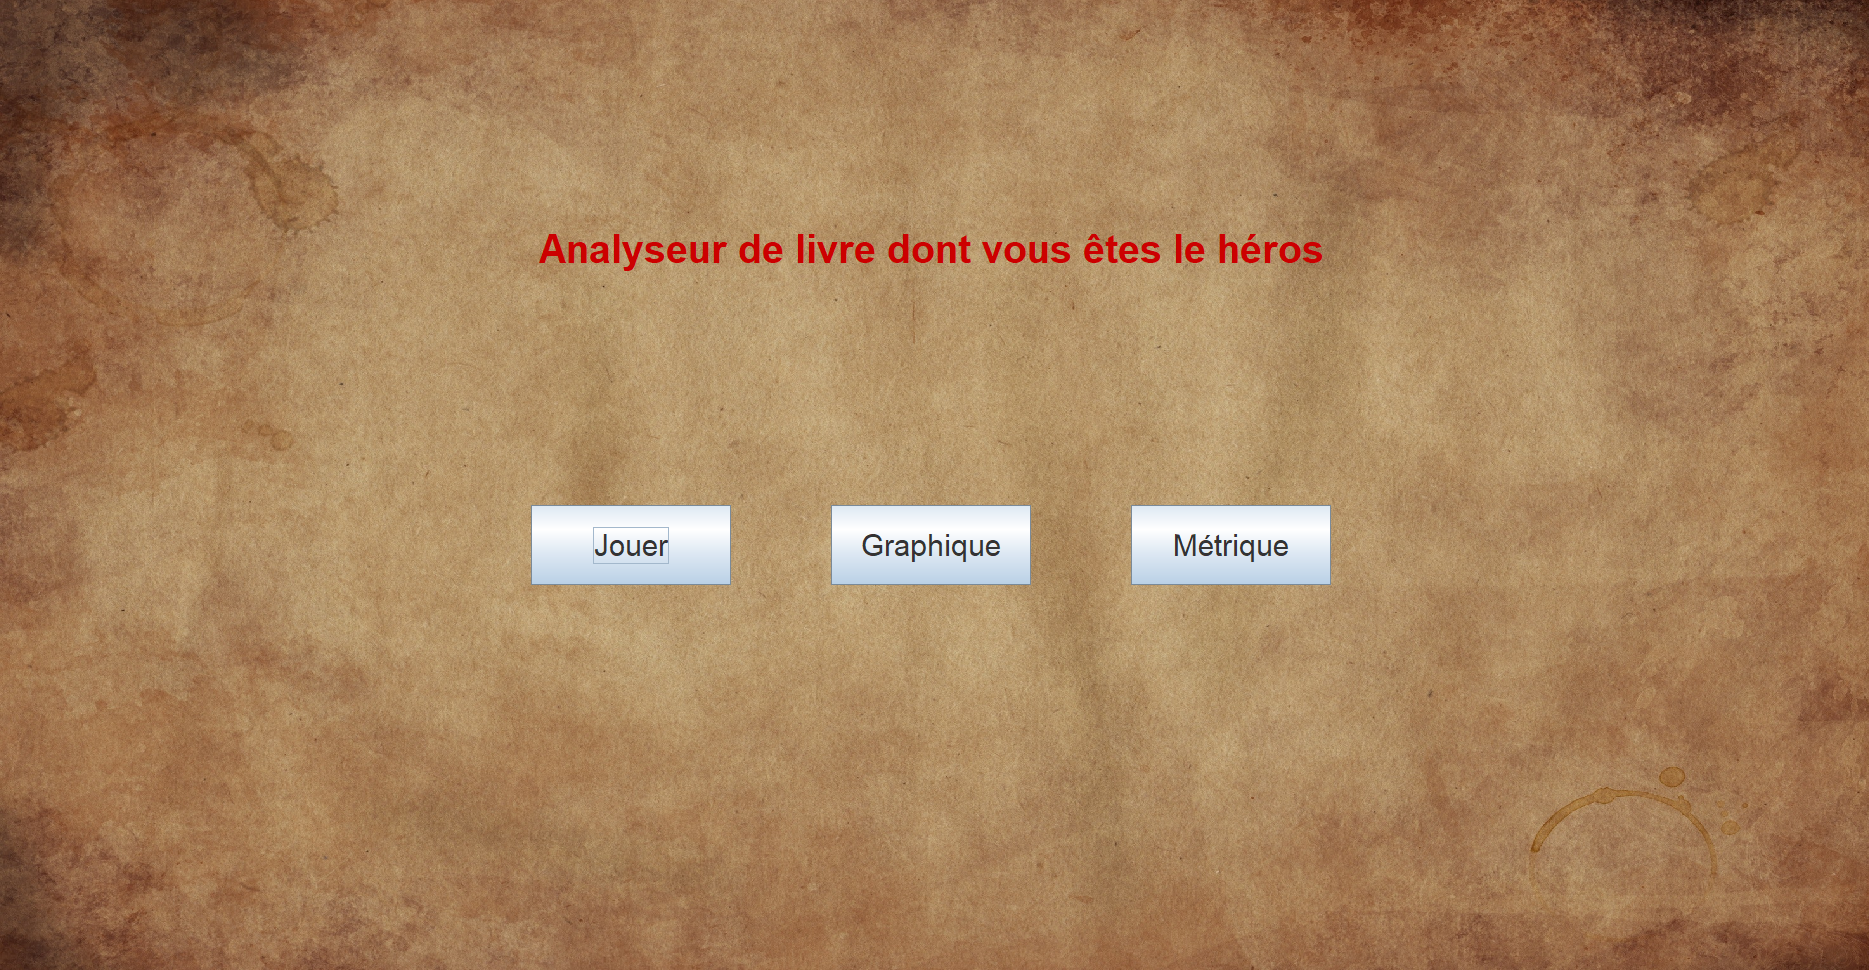
\includegraphics[width=\textwidth]{imgMenu.png}
{\small\textsl{Rendu du menu de l'application.}}
\end {figure}

Une fois le menu passé l'utilisateur arrive sur une des trois parties toutes codées sur la même structure. Chaque partie étend JPanel et est composé elle même de 2 Panel le premier situé en haut contient le bouton de retour au menu et le nom de la partie dans laquelle on se situe et le second sert de Panel de contenu pour la partie. 

\begin {figure}[h]
    \centering
    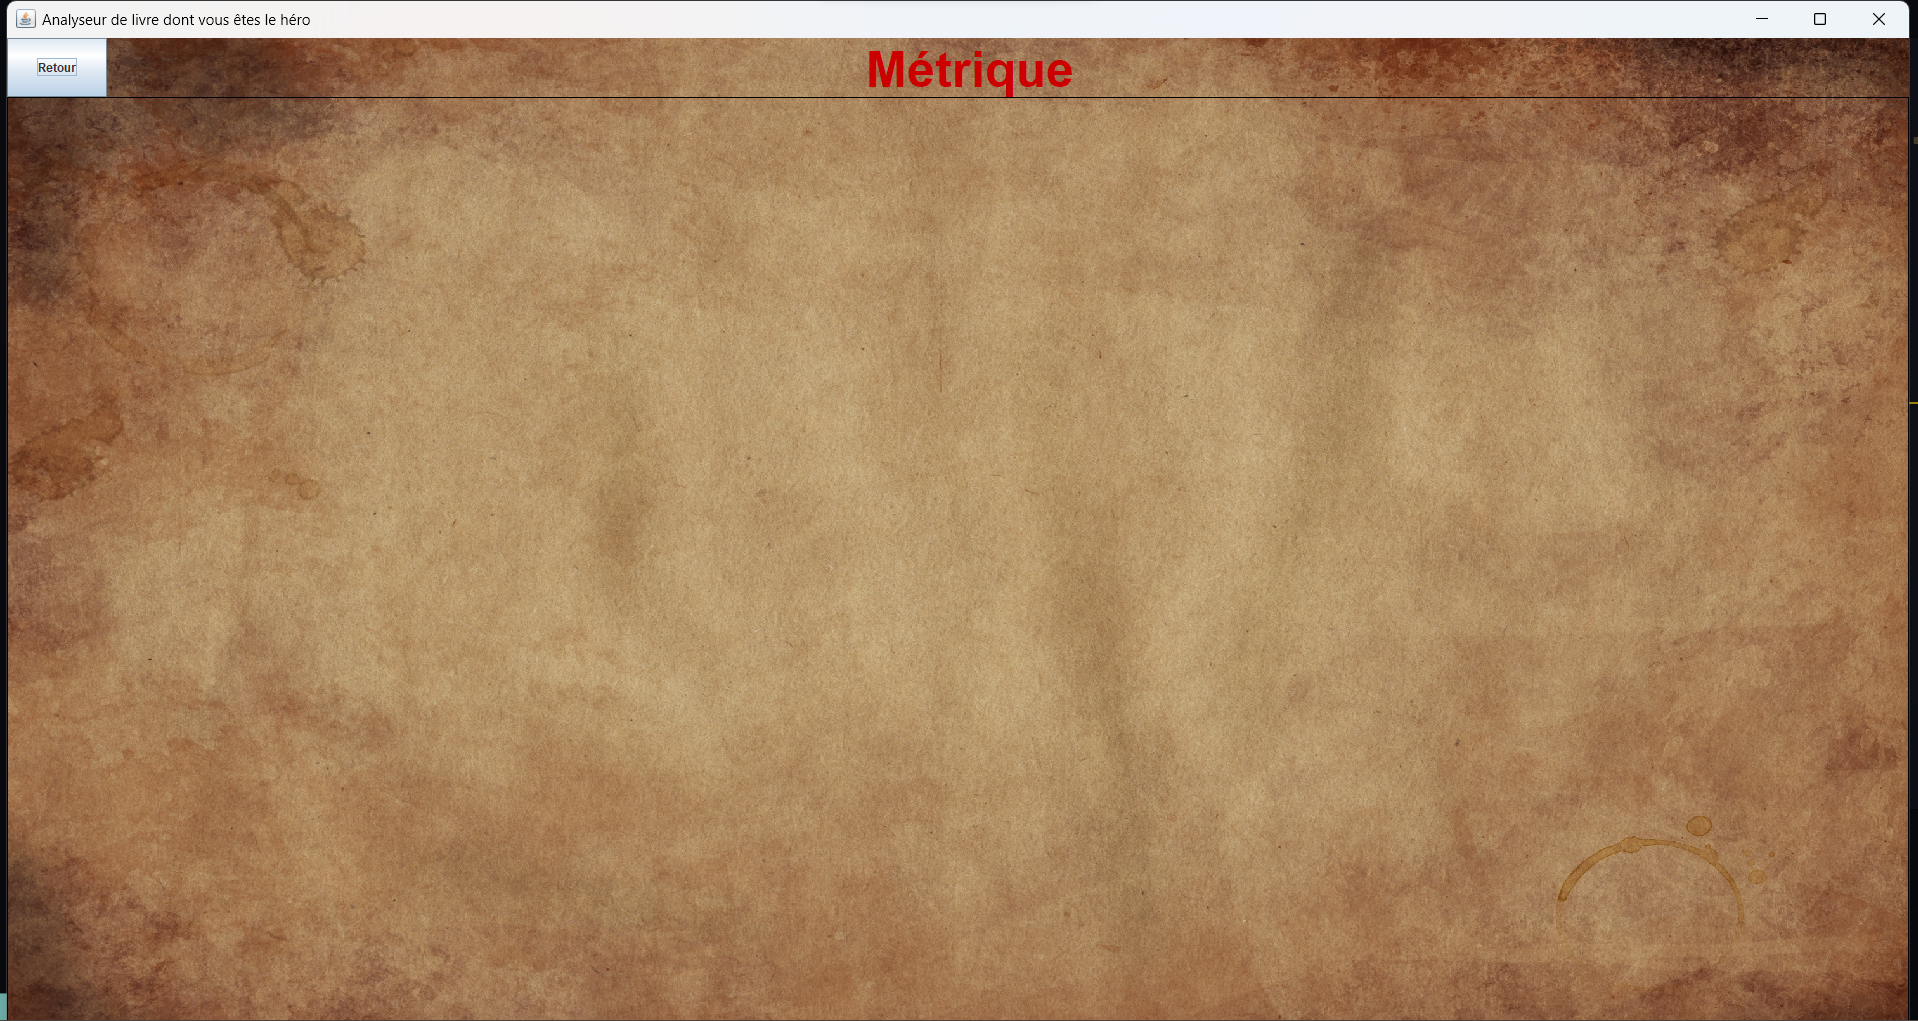
\includegraphics[width=\textwidth]{structureGUI.png}
{\small\textsl{Voici la structure d'une partie avant l'ajout de contenu (une bordure noir a été rajouté afin de délimité les deux JPanel)}}
\end {figure}
\newpage
\subsubsection{Interface de jeu}
La réalisation de l'interface du jeu elle diffère un des autres parties. L'interface graphique doit affiché en temps réel la page sur laquelle le joueur se situe, pour se faire nous avons construit notre application sur le modèle MVC afin de bien respecter l'indépendance de chaque parties. L'interface de jeu est construit sur la même structure que les autres pages avec deux JPanel un principal de contenu et un pour le bandeau supérieur. Dans le JPanel de contenu nous retrouverons deux autres JPanel, le premier qui servira à afficher le texte de la page et un second comportant les boutons pour jouer. 
\begin {figure}[h]
    \centering
    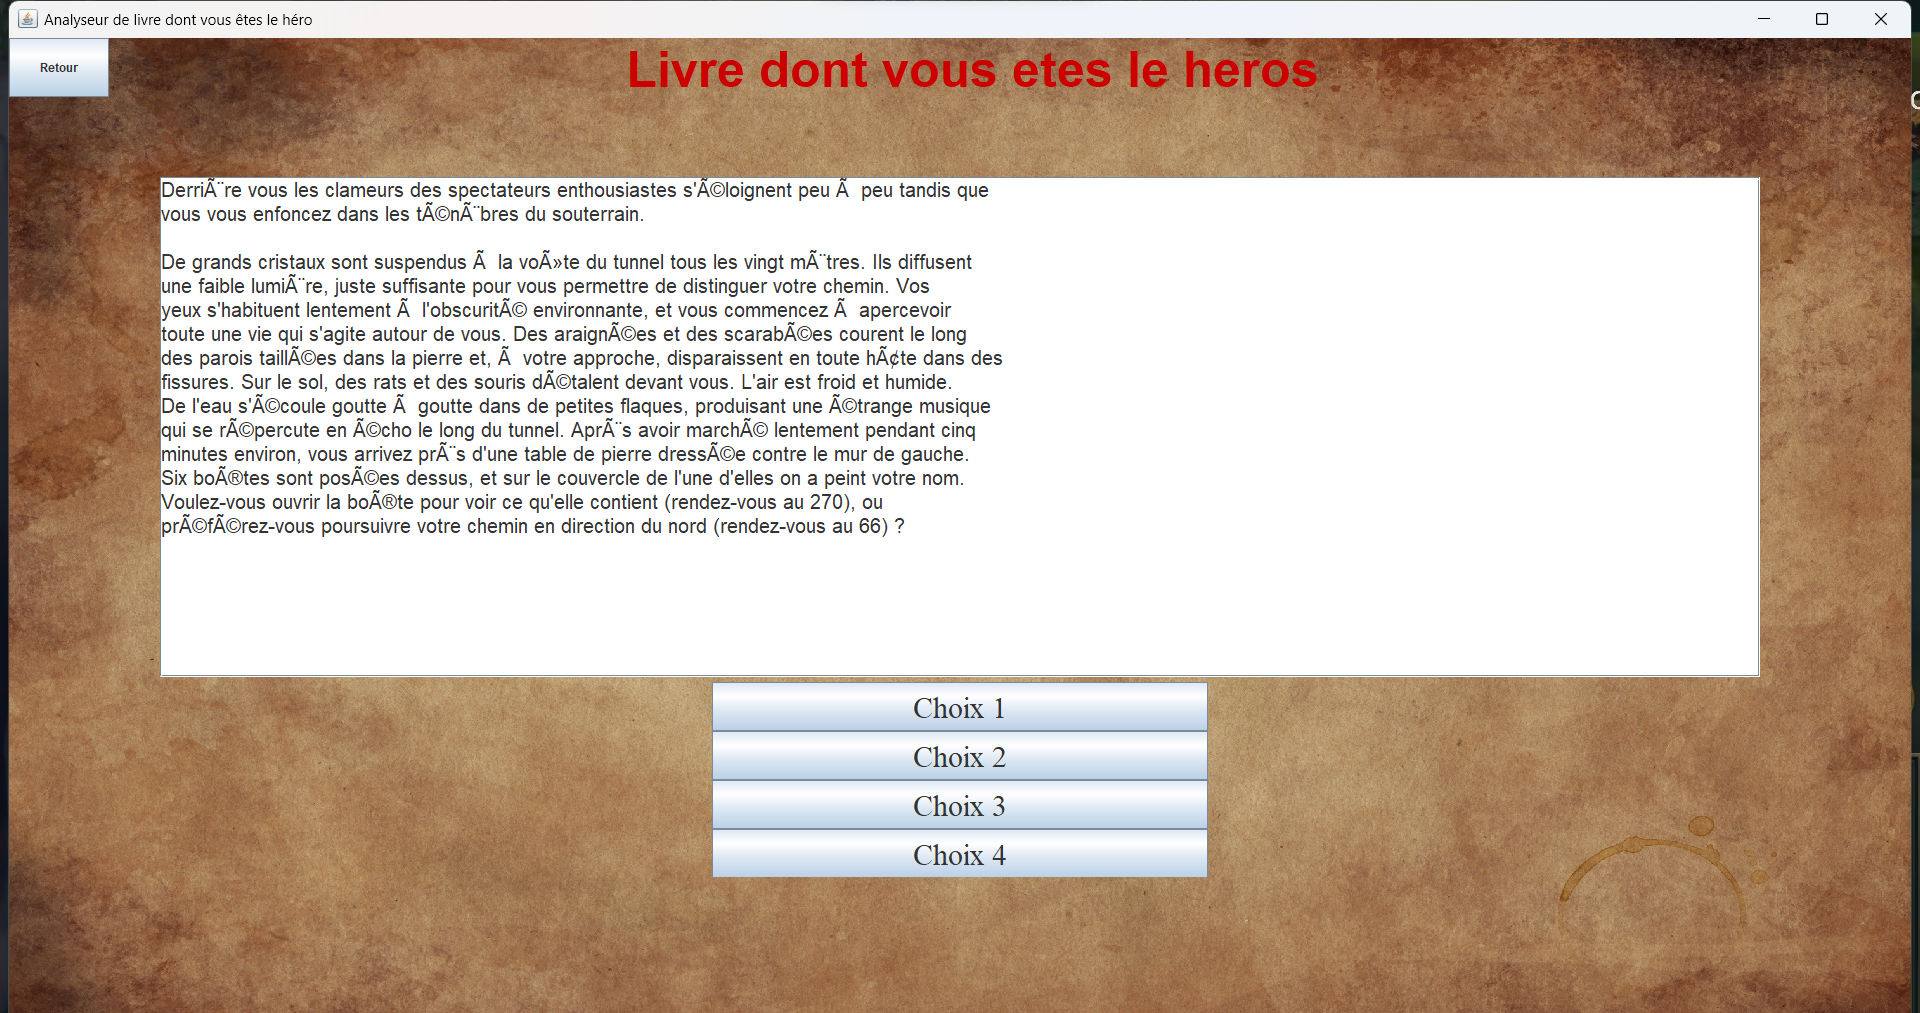
\includegraphics[width=\textwidth]{imgJeu.png}
{\small\textsl{Rendu de la partie jeu de l'application}}
\end {figure}
\newpage
\section{Calcul métrique}
Dans le calcul des métriques, nous avons mesuré les principaux paramètres et statistiques de nos livres, résultant en :\\


\newcolumntype{L}{>{\raggedright\arraybackslash}m{3cm}}
\newcolumntype{C}{>{\centering\arraybackslash}m{1.5cm}}

\begin{table}[h]
\hspace{-1cm}
\begin{minipage}{\textwidth}
\centering
\small
\renewcommand{\arraystretch}{1}
\begin{tabular}{|L|C|C|C|C|C|C|C|C|}
\hline
\textbf{Livre de jeu} & \textbf{\texttt{\#} de Victoires} & \textbf{\texttt{\#} de Fins} & \textbf{\texttt{\#} de Morts} & \textbf{\texttt{\#} de Combats} & \textbf{Chemin le plus court}  & \textbf{Chemin le plus long} & \textbf{Chemin avec le moins de combats} & \textbf{Chemin avec le plus de combats} \\ \hline
FotW.JSON & \vspace{0.4cm}\begin{itemize}
               \item[] 1
           \end{itemize} & \vspace{0.4cm}\begin{itemize}
                             \item[] 20
                         \end{itemize} & \vspace{0.4cm}\begin{itemize}
                                       \item[] 19
                                   \end{itemize} & \vspace{0.4cm}\begin{itemize}
                                                 \item[] 31
                                             \end{itemize} &
                                             \vspace{0.4cm}\begin{itemize}
                                                 \item[] 70
                                             \end{itemize} &
                                             \vspace{0.4cm}\begin{itemize}
                                                 \item[] 82
                                              \end{itemize} &
                                             \vspace{0.4cm}\begin{itemize}
                                                 \item[] 3
                                              \end{itemize} &
                                             \vspace{0.4cm}\begin{itemize}
                                                 \item[] 81
                                             \end{itemize}\\ \hline
                                             
Le-Labyrinthe-de-la-Mort.txt & \vspace{0.4cm}\begin{itemize}
                              \item[] 1
                          \end{itemize} & \vspace{0.4cm}\begin{itemize}
                                        \item[] 35
                                    \end{itemize} & \vspace{0.4cm}\begin{itemize}
                                                  \item[] 34
                                              \end{itemize} & \vspace{0.4cm}\begin{itemize}
                                                            \item[] 21
                                                        \end{itemize} &
                                             \vspace{0.4cm}\begin{itemize}
                                                 \item[] 64
                                             \end{itemize} &
                                             \vspace{0.4cm}\begin{itemize}
                                                 \item[] 81
                                              \end{itemize} &
                                             \vspace{0.4cm}\begin{itemize}
                                                 \item[] 4
                                             \end{itemize} &
                                        \vspace{0.4cm}\begin{itemize}
                                                 \item[] 79
                                             \end{itemize}\\ \hline
\end{tabular}
\caption{Statistiques des livres de jeu}
\end{minipage}
\end{table}


\subsection{Méthodes utilisées pour le calcul des statistiques}
\subsubsection{Agrégation de données}
Le type de calcul utilisé pour les statistiques dans la classe \verb|VictoireMort| est l'agrégation de données.
Le code utilise ce type de calcul pour calculer le nombre de victoires, de morts, de fins et de combats dans un livre. Les calculs sont effectués à travers des méthodes appelées \verb|nbFins()|, \verb|nbMorts()|, \verb|wins()| et \verb|nbCombats()|, qui utilisent des boucles pour parcourir chaque page du livre et effectuer les calculs appropriés.

En particulier, la méthode \verb|nbFins()| compte le nombre de fins dans le livre en vérifiant si chaque page est une fin, \verb|wins| compte le nombre de fins bonnes (c'est-à-dire celles qui mènent à une victoire), \verb|nbMorts()| calcule le nombre de morts en soustrayant le nombre de fins bonnes du nombre total de fins, et \verb|nbCombats()| compte le nombre de pages qui impliquent un combat.
\subsection{Calcul des chemins les plus courts}
\subsubsection{Algorithme de parcours en largeur (Breadth-first search)}
Nous utilisont un algorithme de recherche en largeur (\href{https://en.wikipedia.org/wiki/Breadth-first_search}{BFS} - Breadth-first search) pour explorer tous les chemins possibles dans un livre donné, où chaque page a une ou plusieurs options qui mènent à d'autres pages. La complexité en temps de l'algorithme BFS est O(|V|+|E|), où |V| est le nombre de sommets dans le graphe et |E| est le nombre d'arêtes dans le graphe.

La première méthode \verb|getShortestPathToVictory()| prend deux arguments, \verb|startPage| et \verb|victoryPage|, qui représentent la page de départ et la page de victoire. La méthode utilise une file d'attente pour stocker les chemins possibles à partir de la page de départ. Elle commence par ajouter le chemin initial, qui ne contient que la page de départ, à la file d'attente. Ensuite, elle explore tous les choix possibles à partir de la page courante et ajoute les nouvelles pages atteintes à la file d'attente. Si elle atteint la page de victoire, elle retourne le chemin menant à cette page.

La deuxième méthode \verb|getShortestPathToDeath()| fonctionne de la même manière, mais elle cherche le chemin le plus court depuis la page de départ jusqu'à une page de mort, en vérifiant si la page courante est une page de mort. Si elle atteint une page de mort, elle retourne le chemin menant à cette page. \\ 
\begin{algorithm}[H]
\SetKwInOut{Input}{Entrée}\SetKwInOut{Output}{Sortie}

\Input{Un graphe $G$ et un sommet source $s$}
\Output{Un tableau $dist$ tel que $dist[v]$ soit la distance minimale de $s$ à $v$ dans $G$}

\BlankLine
$visited \gets {}$;
$queue \gets {}$;
$dist[s] \gets 0$;
$visited \gets visited \cup {s}$;
$queue.\mathrm{enfiler}(s)$;

\While{$queue \neq {}$}{
$u \gets queue.\mathrm{defiler}()$;
\ForEach{$v \in G.\mathrm{voisins}(u)$}{
\If{$v \notin visited$}{
$visited \gets visited \cup {v}$;
$dist[v] \gets dist[u] + 1$;
$queue.\mathrm{enfiler}(v)$;
}
}
}

\caption{BFS(G, s)}
\end{algorithm}
\subsection{Calcul des chemins les plus longs}
\subsubsection{Algorithme de parcours en profondeur (Depth-first search)}
Pour calculer le chemin le plus long nous avons utilisé l'algorithme de recherche en profondeur (\href{https://en.wikipedia.org/wiki/Depth-first_search}{DFS} - Depth-first search) dans un livre dont les pages sont reliées par des choix. Le but est de trouver le chemin le plus long de la page de départ à une page de victoire ou de mort, selon la méthode appelée.

Le code utilise une pile (Stack) pour stocker les chemins à explorer. Au début, il ajoute le chemin de départ à la pile, puis commence à explorer les chemins un par un jusqu'à ce qu'il atteigne la page de victoire ou de mort. Pour chaque chemin, il récupère la dernière page visitée, puis examine les choix de cette page. Si la page suivante n'a pas encore été visitée, elle est ajoutée au chemin et placée sur la pile pour une exploration ultérieure.

La méthode \verb|getLongestPathToVictory| prend en entrée deux objets \verb|Page|, la page de départ et la page de victoire, et renvoie la liste des pages dans le chemin le plus long de la page de départ à la page de victoire.

La méthode \verb|getLongestPathToDeath| prend en entrée deux objets \verb|Page|, la page de départ et une liste de toutes les pages du livre, et renvoie la liste des pages dans le chemin le plus long de la page de départ à une page de mort. Cette méthode parcourt les choix dans l'ordre inverse pour garantir que le chemin le plus long vers une page de mort est trouvé en premier. La complexité en temps de l'algorithme DFS est $\mathcal{O}(n + m)$, où |V| $n$ est le nombre de nœuds et $m$ est le nombre d'arêtes dans le graphe.\\
\begin{algorithm}[H]
\caption{DFS (Depth-First Search)}
\SetAlgoLined
\DontPrintSemicolon

\KwIn{un graphe $G=(V, E)$ et un sommet de départ $s \in V$}
\KwOut{un arbre couvrant les sommets atteints depuis $s$}

Marquer le sommet $s$ comme visité;
\ForEach{sommet $v$ adjacent à $s$ non visité}{
Ajouter l'arc $(s, v)$ à l'arbre couvrant;
DFS($G$, $v$);
}
\end{algorithm}


\subsection{Expérimentations dans Métrique}
\subsubsection{Algorithme de Dijkstra}
Dans la partie expérimentale, nous n'avons pas non plus eu peur d'essayer d'utiliser un (\href{https://en.wikipedia.org/wiki/Depth-first_search}{algorithme de Dijkstra}) plus complexe, mais néanmoins plus efficace et plus rentable pour trouver le chemin le plus court vers la victoire et la mort dont la complexité en temps est: $O((|V| + |E|) \log |V|)$ où $|V|$ est un nombre de sommets et $|E|$ est un nombre d'arêtes  dans le graphe en cours de traitement. L'algorithme a une complexité temporelle dans le pire des cas de $O((|V| + |E|) \log |V|)$, où $\log |V|$ représente le temps nécessaire pour les opérations de tas utilisées dans la mise en œuvre de l'algorithme. Dans la class \verb|Experimentations| nous avons une méthode \verb|shortestPathWithLeastCombats|:
Cette méthode calcule le chemin le plus court avec le moins de combats entre une page de départ et une page de victoire. Elle utilise l'algorithme de Dijkstra avec une file de priorité pour choisir les prochaines pages à visiter. La méthode crée également des cartes pour stocker les distances entre les pages, les parents de chaque page et les pages visitées. En tout généralisant, cet algorithme pourrait être beaucoup plus utile si nous avions un code plus complexe, c'est-à-dire calculant des chemins qui ont du poids (super pouvoirs, objets, argent, etc.). Qui aussi pourrait être utiles dans le calcul des probabilités dont on va parler dans la prochaine section.
\subsubsection{Probabilités de gain}
Également dans le dossier \verb|Experimentations|, il y a un test et un exemple de code incomplet pour le calcul des probabilités. Il est resté inachevé en raison d'un petit défaut au niveau des acquisitions virtuelles (nombre de vies, compétences choisies, armes, etc.). En fonction de chacun d'entre eux, à la fin, nous pourrions obtenir la probabilité de la victoire dans chaque page.
\section{Calcul et Graphique}
\subsection{Terminologie}

\subsubsection{Le symbole ":="}
%\cite{"is equal to by definition"}
%\cite{"is defined to be equal to"}
Remplace la valeur actuelle par ce qui suit.

\subsubsection{Graphe simple, non orienté}
Ensemble de nœuds/sommets (vertices) liés entre eux par un ensemble de segments (edges) représentés par une paire de sommets (correspondants respectivement aux deux points constituant le segment.) Le segment (A, B) composé des sommets A et B est équivalent au segment (B, A).

\subsubsection{Graphe orienté}
Même chose qu’un graphe simple à la différence près que les liens entre sommets ont un sens, une direction. On ne les nomme alors plus segment mais vecteurs et ces derniers se définissent de la même manière, sauf que l’ordre de la paire à de l’importance. Le premier sommet marque le début du vecteur, le second la fin. Ce n’est donc plus une paire mais un tuple.


\subsection{Choix de l'algorithme}

\subsubsection{Evaluation du problème}

Nous nous intéresserons à la manière d’afficher une telle structure.

Dans un graphe basé sur un livre dont vous êtes le héros simple : les nœuds correspondent aux paragraphes. Sauf exception, un livre de ce genre est constitué de 300-400 paragraphes et ces derniers peuvent être liés de toutes les façons possibles.

Il existe plusieurs stratégies pour afficher une telle structure. Une partie d’entre-elles associent des forces aux nœuds d’un graphes. Ces dernières influenceront sur leur placement dans l’espace (Principes d’attraction répulsion, ressorts, géométrie ...) Différents modèles sont là encore possibles, tous dirigés vers un certain type de graphe. Ce sont les algorithmes de force.

\subsubsection{Choix de la méthode}

Dans les méthodes présentées dans ce papier, toutes celles tombant sous la catégorie des graphes larges ne vont pas nous intéresser. En effet, un graphe avec 1000 sommets minimum est considéré comme large. Plus la taille de la structure augmente, plus l’algorithme pour la traiter est coûteux. Rien ne sert de tuer la mouche au lance-roquette : Pour des graphes de moins de 500 nœuds, il est donc inutile d’utiliser ces méthodes.

L’inverse est cependant vrai. Tenter d’afficher un graphe plus grand que ce à quoi l’algorithme était destiné peut provoquer des résultats ... aléatoires. Les méthodes de Eades et de Fruchterman-Reynolds sont taillées pour des graphes d’une cinquantaine de sommets seulement. Trop peu en somme.

\subsubsection{La méthode de Tutte}

La méthode de Tutte est, historiquement, la première à obtenir des résultats « corrects » sur des graphes moyens. Aussi appelée la méthode du barycentre, elle s’appuie sur les calculs successifs de ce dernier pour positionner chaque nœud par rapport à ses voisins. Le nombre d’équations à résoudre est proportionnel au nombre de voisins qu’un sommet possède. La complexité correspond donc à la somme des voisins de chaque sommet. Le tout est linéaire. Cependant, il existe des cas où cette méthode génère des graphes sur un espace exponentiellement grand. En effet, en ayant pas imposé de limites à la zone de travail, l’affichage peut en théorie s’étendre sur une surface infinie.

Reste donc l’algorithme de Kamada-Kawai.

\section{L'algorithme de Kamada-Kawai}

\subsection{Visée de l'algorithme}

Kamada et Kawai définissent un affichage désirable de la manière suivante : 
%\cite{"We regard the desirable geometric (Euclidean) distance between two vertices in the drawing as the graph theoretic distance between them in the corresponding graph."}
\textit{(Nous considérons la distance pratique idéale entre deux sommets étant la même que la distance théorique qu’induit le graphe)}

En d’autre termes, la proximité théorique de deux nœuds A B va être conservée à l’affichage.

L’algorithme en lui-même repose sur un principe simple. Les segments reliant les sommets entre eux vont être assimilés à des ressorts. Le positionnement des nœuds est un jeu consistant à équilibrer la force de ces derniers afin d’obtenir une configuration stable. Il faut donc placer chaque nœud de manière à minimiser les forces qu’exerce les ressorts. Ceci est un problème de minimisation.

\subsection{Principe}

\subsubsection{Objectif}

Les objectifs de cet algorithme se résument comme suit : Les nœuds/sommets qui sont proches dans l’idée doivent aussi l’être sur le dessin. Afin de parvenir à rapprocher les sommets qui doivent l’être entre eux, on va poser un système de ressorts sur tous les nœuds du graphe. Les nœuds étant considérés comme proches seront connectés par un ressort d’une grande force, assurant la proximité voulue. A l’inverse, les sommets n’ayant rien à voir entre eux seront reliés par des forces moindres.

\subsubsection{Définition d'un dessin}

En ce qui concerne le dessin en lui-même, quelques qualités précises seront recherchées. L’envie est d’aboutir à un dessin symétrique où les croisements sont minimes et les nœuds distribués de manière uniforme. Comme les critères d’un « bon dessin » restent flous, ces derniers ont été choisi au doigt mouillé comme point de référence. Ici, un dessin est un ensemble de points reliés entre eux par des segments. Les sommets peuvent être placés librement sur un plan carré de taille donnée. Ils ne sont pas restreints à une grille ou autre collection de positions prédéfinies. Voici un exemple de graphe :

\begin{center}
   \begin{tikzpicture}[node distance={15mm}, thick, main/.style = {draw, circle}]
   \node[main] (1) {A};
   \node[main] (2) [below right of=1] {B};
   \node[main] (3) [below left of=2] {C}; 
   \draw (1) -- (2);
   \draw (2) -- (3);
   \end{tikzpicture} 
\end{center}

\subsection{Initialisation}

Avant de pouvoir travailler, il faut se donner un certain nombre de choses.

Soit un graphe $G = \{N, S\}$ avec N l’ensemble des nœuds et S l’ensemble des ressorts.
Soit $|S| = n$ le nombre sommets.
Soit i et j deux sommets quelconques appartenant à G.

On peut donc définir quatre paramètres :
\begin{itemize}
  \item Soit $d_ij$ le plus court chemin entre i et j. (donc la distance)
  \item Soit $l_ij = L * d_ij$ la longueur idéale d’un ressort reliant i et j.
  \item Soit $L = L_0 * diamG$ la longueur désirée des ressorts à l’affichage. (avec L0 la taille de l’espace d’affichage (carré) et diamG : le diamètre du graphe ou la distance entre les sommets les plus éloignés)
  \item Soit $k_ij = \frac{K}{dij^2}$ la force des ressorts entre i et j. (avec K, une constante)
\end{itemize}

Ici, $Lij = L_0 * diamG * dij$.

Ensuite, il faut calculer les choses suivantes :

\begin{enumerate}
  \item La distance $d_ij$ entre tous les sommets du graphe. Ici, constante.
  \item La longueur et la force des ressorts.
  \item Positionner les nœuds sur un polygone régulier à n sommets basé sur un cercle de rayon $L_0$.
\end{enumerate}

\begin {figure}[H]
    \centering
    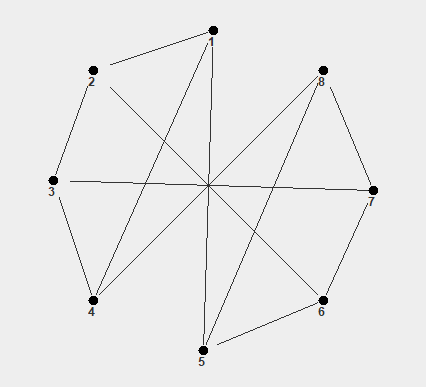
\includegraphics[width=0.5\textwidth]{cube.png}
    \caption{Exemple d'initialisation pour le graphe cube}
\end {figure}

\subsubsection{Matrice de ressorts}

$d_ij$, $l_ij $ et $k_ij$ sont les attributs nécessaires à chaque ressorts. Avant d'entamer la minimisation, il est nécessaire de poser pour chaque paires de points le ressort (ou son absence) les reliants. Toutes ces données sont stockées dans une variante de matrice d'adjacence où en plus des chemins les plus courts, les deux autres données sont stockées dans un objet Ressort. $l_ij $ et $k_ij$ s'obtiennent en fonction de $d_ij$ qui est obtenue via l'algorithme de Floyd-Warshall.


Par exemple pour le graphe à trois points décrit plus haut, voici sa matrice, chaque cellule étant formatée comme suit $(d_{ij} | l_{ij} | k_{ij})$, donnant les valeurs associée au ressort $R_{ij}$ pour toute paire de points $p_i$ et $p_j$. 

$$
\begin{pmatrix}
  (0|0|0) & (1|5|1) & (2|10|\frac{1}{4}) \\
  (1|5|1) & (0|0|0) & (1|5|1) \\
  (2|10|\frac{1}{4}) & (1|5|1) & (0|0|0)
\end{pmatrix}
$$


\subsection{Problèmatique}

On souhaite donc obtenir une disposition de tous les points tel que la fonction d’énergie E soit minime. Il est cependant difficile de trouver un minimum global, de placer tous les points à la fois. On va donc les placer un à la fois en voyant E non pas en tant que fonction de tous les points mais seulement d’un point $p_i$ donné quelconque. Un minimum local se trouve de cette façon. Une valeur de delta $\Delta_i$ est donc associée à chaque point $p_i$. Elle est donnée comme suit :

%delta
$$ \Delta_m = \sqrt{ \left\{\frac{\partial E}{\partial x_m}\right\}^2 + \left\{\frac{\partial E}{\partial y_m}\right\}^2} $$

Ensuite, tant que le delta le plus grand $max_i \Delta_i$ n’est pas en dessous d’un certain seuil, on le réduit puis on revérifie. Et ainsi de suite jusqu’à ce que le plus grand $max_i \Delta_i$ soit en dessous du seuil donné. Une valeur de $\Delta_i$ est associée aux coordonnées de $p_i$. Pour diminuer ou « réduire » cette valeur, il faut donc bouger $p_i$ de façon à trouver les valeurs des coordonnées pour lesquelles $\Delta_i$ est mimime.

\begin{algorithm}[H]
\caption{Pseudo-code de l'algorithme de Kamada-Kawai}\label{alg:cap}
\SetKwInOut{Input}{Entrée}
\SetKwInOut{Output}{Sortie}
\SetKwInOut{Compute}{Compute}
\SetKwInOut{Init}{Initialize}

\Compute{$d_{ij}$ for $1 \leq i \ne j \leq n$}
\Compute{$l_{ij}$ for $1 \leq i \ne j \leq n$}
\Compute{$k_{ij}$ for $1 \leq i \ne j \leq n$}
\Init{$p_1, p_2, ..., p_n$}

\While{$max_i \Delta_i > \mu $}{
let $p_m$ be the particule satisfying $\Delta_m = max_i \Delta_i$;\\
\While{$\Delta_m > \mu $}{
compute $\delta x, \delta y$;\\
$x_m := x_m + \delta x$;\\
$y_m := y_m + \delta y$;
}
}
\end{algorithm}

Il faut donc calculer cette nouvelle position.

\subsubsection{Calcul d'une nouvelle position}

Pour calculer une nouvelle position, une variante de la méthode de Raphson-Newton est utilisée. Cela revient à ajouter aux coordonnées d’un point $p_i$ les solutions $\delta x$ et $\delta y$ en résolvant un système à deux équations de la forme :

\begin{equation}
    \begin{cases}
      a x + b y = c\\
      b x + d y = e
    \end{cases}\
\end{equation}

$$
\text{Où les coefficients}
\begin{cases}
  a = \frac{\partial^2 E}{\partial x^2_m} (x^{(t)}_m, y^{(t)}_m)\\
  b = \frac{\partial^2 E}{\partial x_m \partial y_m} (x^{(t)}_m, y^{(t)}_m) = \frac{\partial^2 E}{\partial y_m \partial x_m} (x^{(t)}_m, y^{(t)}_m)\\
  c = \frac{\partial E}{\partial y_m} (x^{(t)}_m, y^{(t)}_m)\\
  d = \frac{\partial^2 E}{\partial y^2_m} (x^{(t)}_m, y^{(t)}_m)\\
  e = \frac{\partial E}{\partial x_m} (x^{(t)}_m, y^{(t)}_m)
\end{cases}\
$$

Le système résolu n'est pas donné dans le papier original. Une fois résolu, les solutions obtenues sont de la forme :

$$ y = \frac{bc - ea}{b^2 -da} $$
$$ x = \frac{be - dc}{b^2 -da} $$

Ce sont ces dernières qui ont été implémentées.

\subsection{Les dérivées partielles}

Un graphe n’est autre qu’un ensemble de points TT et de RR segments sur lesquels on va venir poser des ressorts.  L’objectif est ici de stabiliser le système afin d’obtenir la répartition la plus équilibrée possible. Dans ce cas, cela se traduit par la minimisation de la force exercée par les ressorts ; ou en d’autres termes, l’énergie totale du système. La somme des forces des ressorts est donnée comme suit :

Soit E la fonction d'énergie du système :
%La fonction d'énergie
$$ E = \displaystyle\sum_{i = 1}^{n - 1} \sum_{j = i + 1}^{n} \frac{1}{2} k_{ij} (|p_i - p_j| - l_{ij})^2 $$

Afin de calculer les positions successives des points, nous allons avoir besoin des dérivées partielles premières et secondes de cette dernière. Elles sont données comme suit dans \href{http://vis.pku.edu.cn/course/Visualization_2018F/reading/drawing_general_undirected.pdf}{le papier original} produit par Kamada et Kawai.

Les dérivées partielles premières :
\begin{equation}
%dEx
\frac{\partial E}{\partial x_m} = \sum_{i \ne m} k_{mi} \left\{ (x_m - x_i) - \frac {l_{mi}(x_m - x_i)}{\{ (x_m - x_i)^2 + (y_m - y_i)^2 \}^{\frac{1}{2}}} \right\}
\end{equation}
\begin{equation}
%dEy
\frac{\partial E}{\partial y_m} = \sum_{i \ne m} k_{mi} \left\{ (y_m - y_i) - \frac {l_{mi}(y_m - y_i)}{\{ (x_m - x_i)^2 + (y_m - y_i)^2 \}^{\frac{1}{2}}} \right\}
\end{equation}

Les dérivées partielles secondes :
\begin{equation}
%dEx2
\frac{\partial^2 E}{\partial x^2_m} = \sum_{i \ne m} k_{mi} \left\{ 1 - \frac {l_{mi}(y_m - y_i)^2}{\{ (x_m - x_i)^2 + (y_m - y_i)^2 \}^{\frac{3}{2}}} \right\}
\end{equation}

\begin{equation}
%dEy2
\frac{\partial^2 E}{\partial y^2_m} = \sum_{i \ne m} k_{mi} \left\{ 1 - \frac {l_{mi}(x_m - x_i)^2}{\{ (x_m - x_i)^2 + (y_m - y_i)^2 \}^{\frac{3}{2}}} \right\}
\end{equation}

\begin{equation}
%dExy
\frac{\partial^2 E}{\partial x_m \partial y_m} = \sum_{i \ne m} k_{mi} \frac {l_{mi}(x_m - x_i)(y_m - y_i)}{\{ (x_m - x_i)^2 + (y_m - y_i)^2 \}^{\frac{3}{2}}}
\end{equation}

\begin{equation}
%dEyx
\frac{\partial^2 E}{\partial y_m \partial x_m} = \sum_{i \ne m} k_{mi} \frac {l_{mi}(x_m - x_i)(y_m - y_i)}{\{ (x_m - x_i)^2 + (y_m - y_i)^2 \}^{\frac{3}{2}}}
\end{equation}

On peut remarquer ici que $\frac{\partial^2 E}{\partial x_m \partial y_m} = \frac{\partial^2 E}{\partial y_m \partial x_m}$. En posant $\Delta x_{mi} = x_m - x_i$, $\Delta y_{mi} = y_m - y_i$ et $ D_{mi} = {\Delta x_{mi}}^2 + {\Delta y_{mi}}^2 $, les expressions se simplifient alors de la manière suivante :

Les dérivées partielles premières :
\begin{equation}
%dEx
\frac{\partial E}{\partial x_m} = \sum_{i \ne m} k_{mi} \left\{ \Delta x_{mi} - \frac {l_{mi}\Delta x_{mi}}{D_{mi}^{\frac{1}{2}}} \right\}
\end{equation}
\begin{equation}
%dEy
\frac{\partial E}{\partial x_m} = \sum_{i \ne m} k_{mi} \left\{ \Delta y_{mi} - \frac {l_{mi}\Delta y_{mi}}{D_{mi}^{\frac{1}{2}}} \right\}
\end{equation}

Les dérivées partielles secondes :
\begin{equation}
%dEx2
\frac{\partial^2 E}{\partial x^2_m} = \sum_{i \ne m} k_{mi} \left\{ 1 - \frac {l_{mi}{\Delta y_{mi}}^2}{D_{mi}^{\frac{3}{2}}} \right\}
\end{equation}
\begin{equation}
%dEy2
\frac{\partial^2 E}{\partial y^2_m} = \sum_{i \ne m} k_{mi} \left\{ 1 - \frac {l_{mi}{\Delta x_{mi}}^2}{D_{mi}^{\frac{3}{2}}} \right\}
\end{equation}

\begin{equation}
\frac{\partial^2 E}{\partial x_m \partial y_m} = \sum_{i \ne m} k_{mi} \left\{ \frac {l_{mi} \Delta x_{mi} \Delta y_{mi}}{D_{mi}^{\frac{3}{2}}} \right\}
\end{equation}

Les sommes de ces dernières peuvent enfin être factorisées sous la forme $k_{mi} \left\{ a - \frac {l_{mi}b}{D_{mi}^p} \right\}$ permettant ainsi une implémentation aisée.

\subsection{Exemple témoin}

Voici un exemple d'application sur le graphe témoin, de diamètre 2, sur un plan de 10 par 10.

\begin {figure}[H]
    \centering
    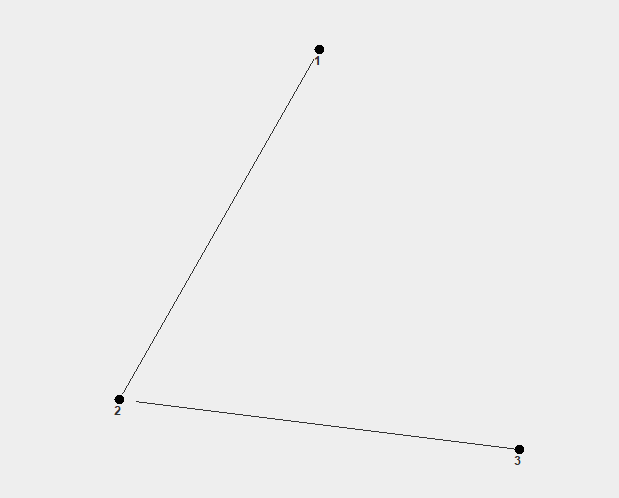
\includegraphics[width=0.9\textwidth]{temoin.png}
    \caption{Graphe témoin}
\end {figure}

On initialise A, B, C (1, 2, 3) sur un cercle de rayon 10 et de centre 5. Donc on a $\{A(5, 0), B(1, 7), C(9, 8)\}$. Les ressorts $AB = BA$ étant égaux, on ne s'intéresse qu'aux ressorts de la moitié inférieure de la matrice symétrique. Il s'agit donc de sommer AB et BC. 

\subsection{Résultats}

\subsubsection{Visualisation}

Niveau interface graphique, un module entier de consultation de graphe a été réalisé. Il est possible de visualiser le dessin d’un graphe tel que décrit plus haut. Si ce dernier dépasse, il est possible de faire dérouler l’écran pour le voir en entier. Par défaut, un graphe est initialisé en cercle. Il est possible de choisir via le menu à gauche d’appliquer l’algorithme de Kamada et Kawai. Il est tout à fait possible d’y ajouter d’autres algorithmes/modes de calcul. L’option de zoomer est implémentée dans le code mais n’est pas disponible via l’interface (ceci est notamment utilisé sur le graphe témoin. A l’origine fait pour un plan de 10*10, cela correspondait à un plan de 10*10 pixels en pratique et était de ce fait trop petit pour être vu. La place pour afficher les points et les segments n’y était pas. Ce zoom qui n’est autre qu’un facteur multiplicatif s’est donc avéré nécessaire). C’est une autre possibilité d’évolution.

\begin {figure}[H]
    \centering
    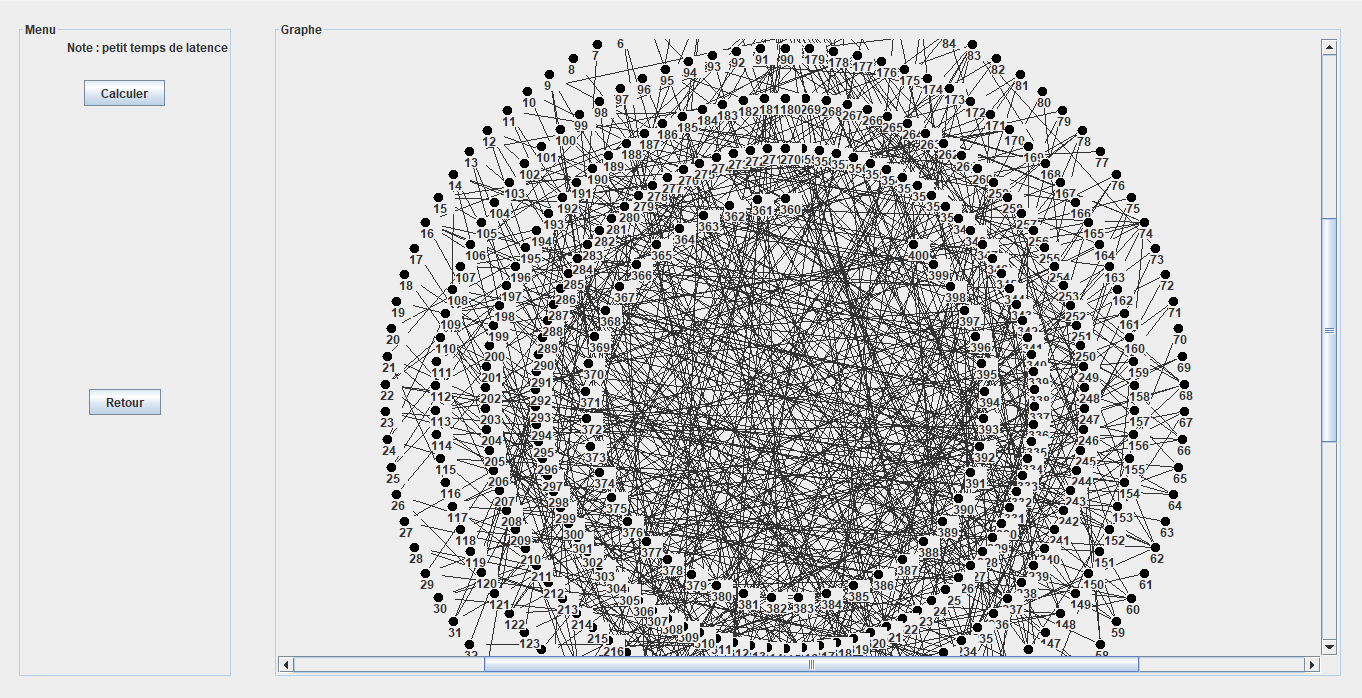
\includegraphics[width=0.9\textwidth]{interface.png}
    \caption{Interface de visualisation avec graphe texte}
\end {figure}

Avant d’arriver sur l’écran de visualisation, un menu avec plusieurs choix de graphe se présente. \textbf{Graphe Txt} et \textbf{Graphe Json} sont respectivement les graphes associés aux livres format texte et format json utilisés pendant le développement. Il est possible d’ajouter d’autres presets. \textbf{Graphe Témoin} est le graphe sur lequel les calculs de référence pour l’implémentation de Kamada Kawai ont été menés. \textbf{Graphe Cube} correspond à un cube en trois dimensions. Cet exemple est directement tiré du papier original de Kamada et Kawai et permet d’attester du fonctionnement de l’algorithme.

\begin {figure}[H]
    \centering
    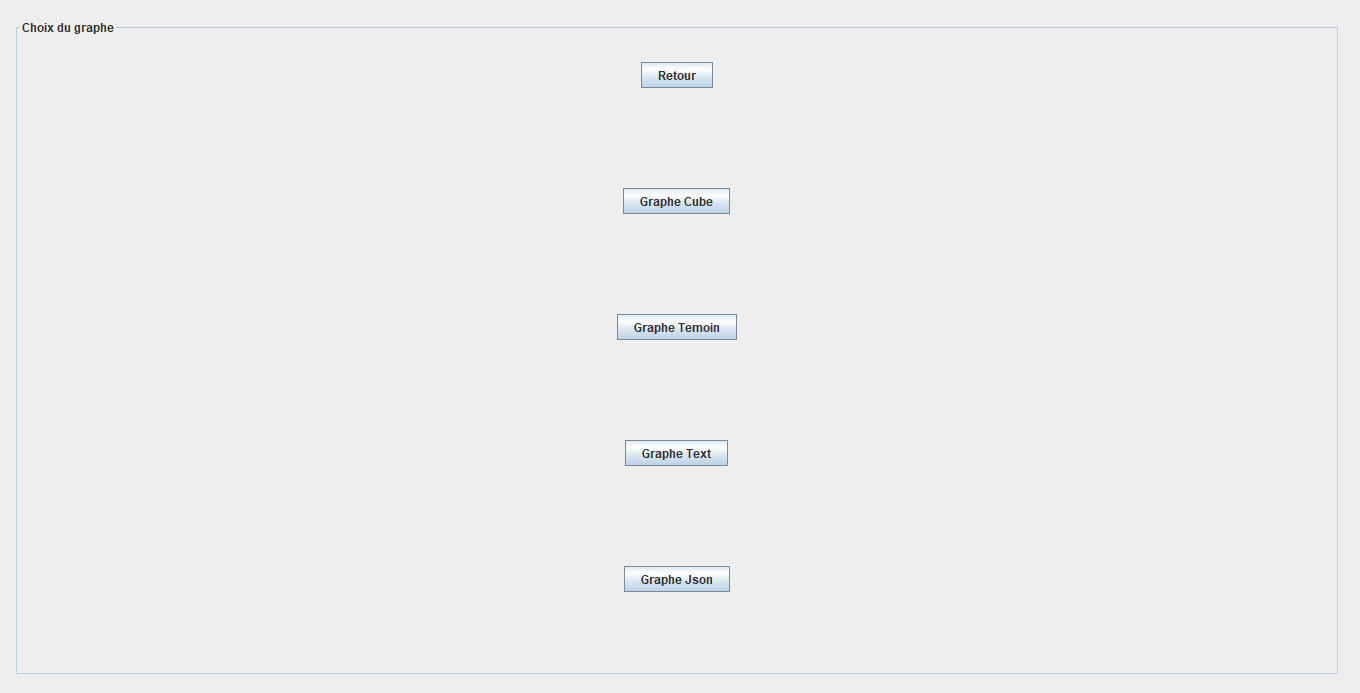
\includegraphics[width=0.9\textwidth]{choix_graphe.png}
    \caption{Choix des différents graphes}
\end {figure}

\subsubsection{Limitations}

Pour attester du fonctionnement de l’algorithme, des graphes ont été utilisés comme point de comparaison. Un graphe témoin, servant de référence pour la compréhension des calculs et leur simplification à l’implémentation. Sans surprise, les résultats obtenus à la main correspondent aux résultats encodés. C’est tout le but d’un témoin. Ce graphe en particulier a été choisi de manière à simplifier les calculs.

\begin{figure}[H]
\centering
\begin{subfigure}{.5\textwidth}
  \centering
  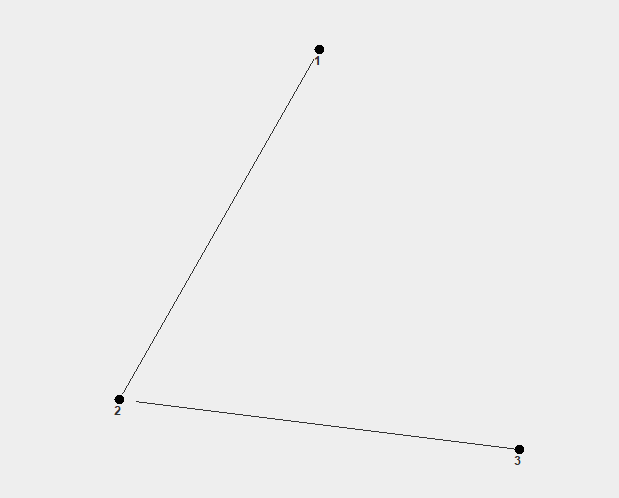
\includegraphics[width=.5\linewidth]{temoin.png}
  \caption{Initialisation}
  \label{fig:Sub1}
\end{subfigure}%
\begin{subfigure}{.5\textwidth}
  \centering
  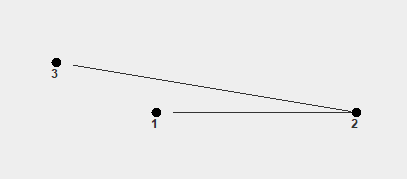
\includegraphics[width=.5\linewidth]{temoin_err.png}
  \caption{Résultat obtenu}
  \label{fig:sub2}
\end{subfigure}
\caption{Application au graphe témoin}
\label{fig:test2}
\end{figure}

Cependant, la difficulté de ne prendre que ce graphe comme référence est qu’il n’y a pas d’attente sur le résultat, donc aucun moyen d’attester de sa validité. Entre donc le cube :

\begin{figure}[H]
\centering
\begin{subfigure}{.5\textwidth}
  \centering
  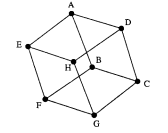
\includegraphics[width=.5\linewidth]{cube_des.png}
  \caption{Résultat attendu}
  \label{fig:sub3}
\end{subfigure}%

\begin{subfigure}{.5\textwidth}
  \centering
  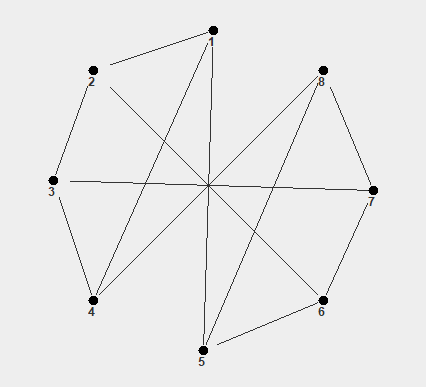
\includegraphics[width=.5\linewidth]{cube.png}
  \caption{Initialisation}
  \label{fig:sub4}
\end{subfigure}

\begin{subfigure}{.5\textwidth}
  \centering
  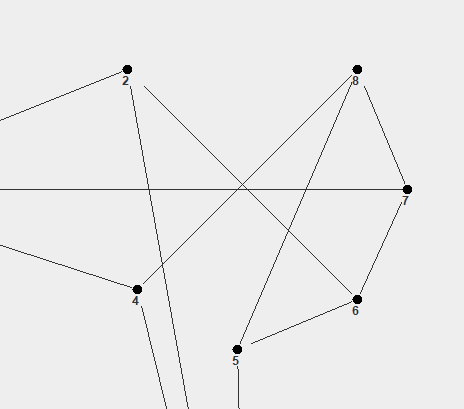
\includegraphics[width=.5\linewidth]{cube_err.png}
  \caption{Résultat obtenu}
  \label{fig:sub5}
\end{subfigure}

\caption{Application au cube}
\label{fig:test}
\end{figure}

Et ... Oui. Cela ne marche pas. Même en recodant le tout à deux reprises, le même problème se pose. Pour stopper un calcul, il faut que les deltas soient sous un certain seuil, or il arrive que les deltas, réduits individuellement, ne passent jamais ce seuil. Cela se traduit de deux façons :

\begin{itemize}
  \item Le calcul des positions successives converge vers un ensemble de valeurs pour ne plus en sortir. Certaines fois, dans le processus de minimisation, les valeurs à l’origine proche du seuil bondissent vers un ordre supérieur et y restent, faute de pouvoir les réduire (rencontre d’une boucle). Dans le cas où elles passent bien sous le seuil, le temps de calcul s’en retrouve tout de même grandement affecté (augmentation conséquente pour rien).
  \item Les points sont positionnés à tour le rôle aux mêmes positions atteignant de ce fait une répartition stable. Néanmoins comme leurs deltas ne sont pas en dessous du seuil, le positionnement successif continue et boucle à l’infini en une sorte de jeu de chaises musicales.
\end{itemize}

En outre, plus le seuil est éloigné du plus grand delta $max_i \Delta_i$ à l’initialisation, plus le calcul prend du temps, si toutefois il se termine sans rencontrer de boucle infinie. Sur les graphes de grande envergure, cela boucle systématiquement. En l’état, il faut donc choisir un seuil proche $max_i \Delta_i$ et espérer au mieux... !

\section{Mot de la fin}

Pour conclure, visualiser des réseaux de données n’est pas chose aisée. Les critères formant un bon dessin sont plus que relatifs. Cependant, en s’accordant sur des principes généraux, il est possible de définir un cadre pour un affichage optimal.
Tout d’abord, une interface pour voir tout système de points reliés entre eux a été réalisée. Ensuite, s’est posé la question de leur positionnement. Dans un premier temps, un algorithme d’initialisation simple a été fait. Dans un second temps, l’implémentation d’un algorithme plus complexe (Kamada Kawai) a été tentée. Cette dernière étape n’a peut-être pas abouti, néanmoins le processus de développement a donné son lot de jolies choses.

\begin {figure}[H]
    \centering
    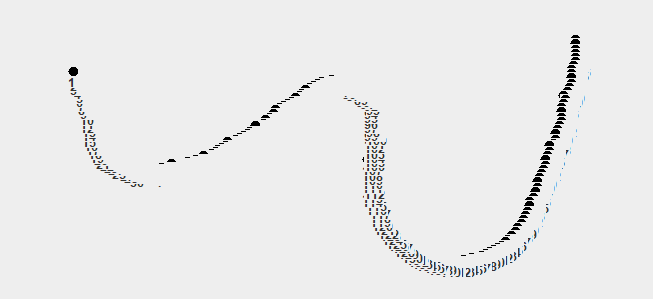
\includegraphics[width=0.9\textwidth]{serpent.png}
\end {figure}

\section{Ressources utilisées}

\subsection{Partie graphe}

\begin{itemize}

  \item \href{http://asus.myds.me:6543/paper/ktall/Z\%202431\%20-\%201989\%20-\%20AN\%20ALGORITHM\%20FOR\%20DRAWING\%20GENERAL\%20UNDIRECTED\%20GRAPHS.pdf}{Z 2431 - 1989 - AN ALGORITHM FOR DRAWING GENERAL UNDIRECTED GRAPHS}
  \item \href{https://www.programiz.com/dsa/floyd-warshall-algorithm#:~:text=Floyd\%2DWarshall\%20Algorithm\%20is\%20an,in\%20a\%20cycle\%20is\%20negative}{Floyd-Warshall Algorithm}
  \item \href{https://cs.brown.edu/people/rtamassi/gdhandbook/chapters/force-directed.pdf}{Force Directed Drawing Algorithms}
  \item \href{https://www.stashofcode.fr/rotation-dun-point-autour-dun-centre/}{Rotation d'un point autour d'un centre}
  \item \href{https://en.wikibooks.org/wiki/LaTeX/Mathematics}{Latex/Mathematics}
  \item \href{https://www.baeldung.com/cs/latex-drawing-graphs}{Draw a Graph Using LaTeX}
\end{itemize}
\section{Conclusion}
Le projet fut enrichissant pour chacun d'entre nous. Il nous a permis d'améliorer nos compétences en programmation orienté objet en java. Nous avons pu développer une première application avec une interface graphique. Mais ce projet fut aussi stimulant et nous a permis de mieux comprendre les problématiques liés aux travaux de groupes. La communication, pouvoir expliquer ce que l'on compte coder afin que les autres puissent commencer sur leurs parties respectives, ou même les problèmes liés a l'implémentation du code des autres furent des épreuves que nous avons du surmonter afin de mener ce projet à bout. Le projet pourrait néanmoins être largement améliorer sur certains points. 


\end{document}
